\begin{recipe}
[ %
	preparationtime = {\SI{2}{\hour} (overnight raise)},
%	bakingtime={\SI{1}{\hour}},
%	bakingtemperature={\protect\bakingtemperature{topbottomheat=\SI{280}{\celsius}}},
	portion = {\portion[Pizza]{2}},
	source = {BrainStew},
	sourceref = {\href{https://www.seriouseats.com/recipes/2010/09/hacker-free-neapolitan-pizza-for-a-home-kitchen-recipe.html}{Serious Eats}}
    ]{Neapolitan Pizza Dough in/on your Oven}

	\begin{figure}[p]
		\centering
		\makebox[\textwidth][c]{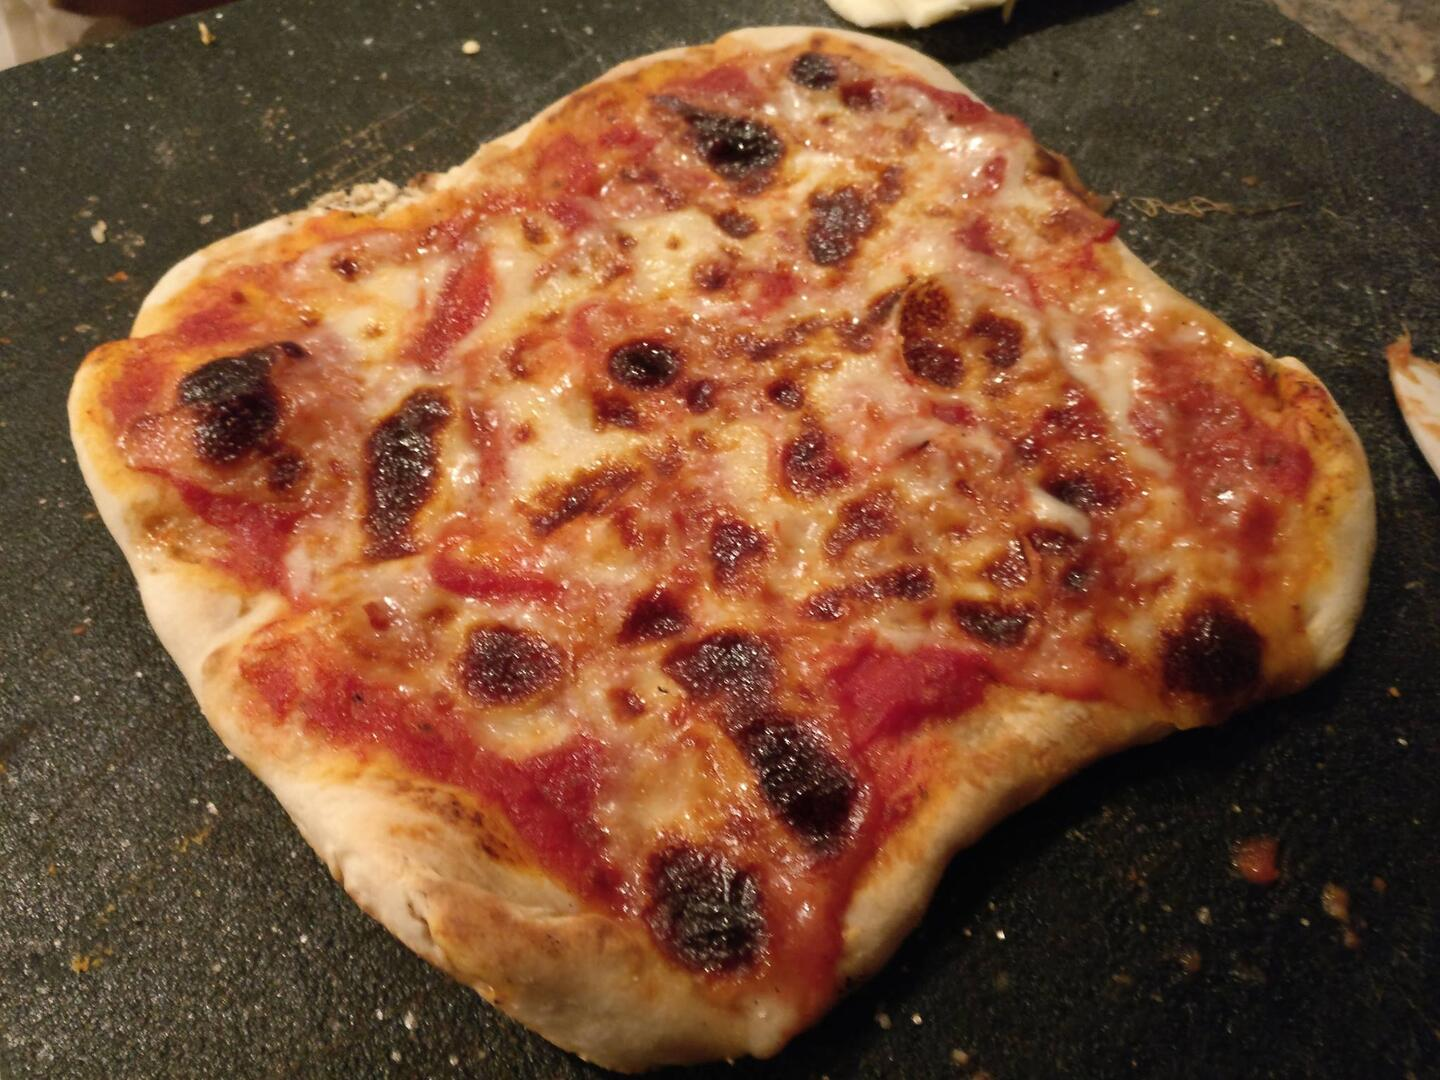
\includegraphics[height=\textheight]{neapolitan_pizza_dough/QAggM5x.jpg}}
	\end{figure}

    \introduction{
    	If you are making pizza for a group, double this recipe at least. The written proportions will feed 1--2 people depending on how much pizza those people eat.

    	\textbf{Special Equipment:}
    	A cast iron skillet. Larger skillets will make bigger pizzas.
	}

	\ingredients[]{
		\SI{20}{\ounce} (\SI{4}{cups}) &  Flour, ideally 00 but standard all purpose or bread flour is fine \\
		\SI{0.3}{\ounce} (about \SI{2x1/4}{\teaspoon}) & Kosher salt \\
		\SI{0.2}{\ounce} (about \SI{1}{\teaspoon}) & Instant yeast \\
		\SI{0.2}{\ounce} (about \SI{2}{\teaspoon}) & Sugar \\
		\SI{12}{\ounce} & Water \\
		& Semolina (optional) for sprinkling
	}

	\preparation{
		\step Combine/whisk the dry ingredients together. Either by hand, or with a mixer and a dough hook attachment, slowly add in the water until no dry flour remains. Let the dough rest for \SI{10}{\minute}.

		\step After the rest, keep kneading the dough until a sticky dough that barely pulls away from the bowl sides forms. This should take around \SI{10}{\minute}. You may need more water, or more flour. Add just a little flour at a time (a tablespoon or so) if the dough is too wet.

		If you’re unsure if the dough is finished, you can try the window-pane method. Let the dough rest for a couple of minutes, then tear away a small ball. Try stretching this small ball into a thin sheet using your fingertips. If you can almost see through it like a window pane before any holes form, then you’re good to go. Otherwise, knead for 5 more ``turns'' and let rest again to check.

		\step Roll this dough up into a tight ball, lightly oil and place in either a large bowl with a tight cover or divide into a couple of ziptop bags. Leave the dough out on the counter overnight, or put into the fridge for up to \SI{72}{\hour}. If you are going the counter route, make sure your dough has room to expand up to $3\times$.

		\step When you are ready to use your dough, turn on the broiler in your oven and put one rack at the highest spot, or if your oven doesn't have a broil setting preheat your oven to the highest temperature.

		\step Prepare your toppings. Neapolitan pizzas traditionally have chunks of buffalo or fresh mozzarella, hand crushed canned tomatoes with a little salt and pepper, some fresh basil, and a drizzle of good olive oil. But you do you! If you are going with fresh mozzarella, make sure to dry it out a bit by pressing it between two paper towels under a heavy plate. You may want to strain your canned tomatoes as well to reduce soupiness.

		\step Stretch your dough into a thin disk that just fits into your cast iron. This style of pizza is not meant to have a very thick crust, but try to avoid having any holes in the dough. You may not need all of the dough for one pizza, so split it as needed.

		\step Heat your cast iron to the highest temperature that won't cause your fire alarm to go off on the stove.

		\step Once the pan is very hot, sprinkle some semolina or standard flour on it, and drop your dough disk onto the flour. Let the dough cook until the bottom has just started to get some brown color to it, but isn't fully browned.

		\step Quickly top your pizza. You can do this while the dough is cooking, but it does make checking the bottom side of the dough a bit harder to pull off without making a mess.

		\step Pop your pizza into the top of your oven, directly underneath the broiler if using it. Keep an eye on it during this process, and turn the pan or move it further from the heat to avoid burning. Once the crust on top has browned nicely, you have yourself a delicious pizza!
	}

\end{recipe}